\chapter{Representing Images and Geometry}
\label{chapter:geometry_homogeneous}

%\chapter{Imaging Geometry}

%\reviewcomment{Chapter partially completed. References missing. Several figures missing. Side notes missing.}

%\reviewcomment{Question: this chapter could go much later, should it go inside  visual understanding part? That is closer to the applications when this material will become useful.}

%For many computer vision tasks, we need to know the relationship between the positions of points in the world and where they appear in the image taken by a camera.  Determining those relationships, which involves both measuring properties of a camera and also its position and orientation, is called {\em camera calibration}. To perform the calculations needed for camera calibration it is convenient to use a set of coordinates known as homogeneous coordinates.

%In this chapter we will introduce the formulation that is commonly used when studying scene geometry.

\section{Introduction}


Before we dive into the material of this chapter, let's start by questioning the way in which we have been representing images up to now. In most of the chapters, we have represented images as ordered arrays of pixel values, each pixel described by its grayscale value (or three arrays for color images). We will call this representation the {\bf ordered array}.
\begin{equation}
\boldimg = 
\left[
\begin{matrix}
\img [1,1] & \dots & \\
\vdots & \img [n,m] & \vdots \\
 & \dots  & \img [N,M] \\
\end{matrix}
\right]
%\left[x [n,m] \right]
\end{equation}
Each value is a sample on a regular spatial grid. In this notation $s$ represents the pixel intensity at one location. This is the representation we are most used to and the typical representation used when taking a signal processing perspective. It makes it simpler to describe operations such as convolution.

However, an image can be represented in different ways, making explicit certain aspects of the information present on the input. What else could we do to represent an image? Another very different, but equivalent, representation is to encode an image as a collection of points, indicating its color and location explicitly. In this case, an image is represented as a {\bf set of pixels}:
\begin{equation}
\left\{ [\img_i,x_i,y_i] : i \right\}
\label{eq:set_of_pixels}
\end{equation}
 where $\img_i$ is the pixel intensity (or color) recorded at location $(x_i,y_i)$. 
 This representation makes the geometry explicit. It might seem like a trivial representation but it makes some operations easy (and others complex). For instance, we can apply geometric transformations easily by directly working with the spatial coordinates. Imagine you want to translate an image, described by \eqn{\ref{eq:set_of_pixels}}, to the right by one pixel, you can do that easily by simply creating the new image defined by the set of translated pixels: $\left\{ [\img_i,x_i+1,y_i] : i \right\}$. 

 \marginnote{Representing images as sets of points is very common in geometry-based computer vision. We will use this representation extensively in the following chapters.}
 
 Although both previous representations might seem equivalent, the set representation makes it easy to deal with other image geometries where the points are not on a regular array. 
 
 That representation can also be extended by representing geometry in different ways such as using homogeneous coordinates, or positional encoding. We will discuss homogeneous coordinates in this chapter. 

The previous two representations are not the only ways in which we can represent images. Another option is to represent an image as a continuous function whose input is
a location $(x, y)$ and it output is an intensity, or a color, $\img$:
\begin{equation}
   \img (x,y) = f_{\theta}(x,y)
\end{equation}
This image representation is commonly used when we want to make image priors more explicit. The function $f_{\theta}$ is parameterized by the coefficients $\theta$. This function becomes especially interesting when the parameters $\theta$ are different than the original pixel values. They will have to be estimated from the original image. But once learned, the function $f$ should be able to take as input continuous spatial variables.

These three representations induce different ways of thinking about architectures to process the visual input. These representations are not opposed and can be used simultaneously.

The ordered array of pixels is the format that computers take as input when visualizing images. However, a set of pixels is the most common format when thinking about three-dimensional (3D) geometry and image formation. Therefore, it is always important to be familiar with how to transform any representation into an ordered array.

%Let's start by studying some two-dimensional (2D) geometric image transformations and we will use them as a excuse to introduce homogeneous coordinates. %Homogeneous coordinates will become very important when talking about 3D geometry and 2D image formation. 

We will start by introducing homogeneous coordinates, an important tool that will simplify the formulation of perspective projection. 


\section{Homogeneous and Heteregenous Coordinates}


Homogeneous coordinates represent a vector of length $N$ by a vector of length $N+1$.
The transformation rule from heterogeneous to homogeneous coordinates is simply to add an additional coordinate, 1, to the heterogeneous coordinates as shown here:
\begin{equation}
    \begin{pmatrix}
    x \\
    y 
    \end{pmatrix}
    \rightarrow 
    \begin{bmatrix}
    x \\
    y \\
    1
    \end{bmatrix}
    \label{eq:2dhomo}
\end{equation}
It is the same if the vector has three dimensions:
\begin{equation}
    \begin{pmatrix}
    x \\
    y \\
    z
    \end{pmatrix}
    \rightarrow 
    \begin{bmatrix}
    x \\
    y \\
    z \\
    1
    \end{bmatrix}
    \label{eq:3dhomo}
\end{equation}


We will refer to conventional Cartesian coordinate descriptions of a point in 2D, such as $(x,y)$, or 3D, such as $(x,y,z)$, as {\bf heterogeneous coordinates} and write with rounded brackets in this chapter.  We denote their corresponding {\bf homogeneous coordinate} representations by square bracketed vectors.

\marginnote{August Ferdinand Möbius, a German mathematician and astronomer, introduced homogeneous coordinates in 1827. He also cocreated the famous Möbius strip.}

The homogeneous coordinates have the additional rule that all (non-zero) scalings of a homogeneous coordinate vector are equivalent.  For example, to represent a 2D point, we have (transforming from heterogeneous to homogeneous coordinates),
\begin{equation}
    %(x,y) \rightarrow 
    \begin{bmatrix}
    x \\
    y \\
    1
    \end{bmatrix}
    \equiv 
    \begin{bmatrix}
    \lambda x \\
    \lambda y \\
    \lambda
    \end{bmatrix}
\end{equation}
for any non-zero scalar, $\lambda$. To go from homogeneous coordinates back to the heterogeneous representation of the point, we divide all the entries of the homogeneous coordinate vector by their last dimension:

\begin{equation}
    \begin{bmatrix}
    x \\
    y \\
    w
    \end{bmatrix}
    \rightarrow 
    \begin{pmatrix}
    x/w \\
    y/w 
    \end{pmatrix}
\end{equation}

\Fig{\ref{fig:homogeneousAndHeteregeneous}} illustrates how homogeneous and heterogeneous coordinates relate to each other geometrically. A point in homogeneous coordinates is scale invariant (any point within the line that passes through the origin translates into the same point in heterogeneous coordinates). We can already see that this is closely related to the operation performed by perspective projection. 

\begin{figure}
\centerline{
\includegraphics[width=0.7\linewidth]{figures/imaging_geometry/homogeneousAndHeteregeneous_VS3.eps}
}
\caption{Transformation rule between heterogeneous and homogeneous coordinates in 2D. All the points along the dotted line correspond to the same point in heterogeneous coordinates. Note that the points $(x,y)$ and $(x,y,1)$ live in different spaces.}
\label{fig:homogeneousAndHeteregeneous}
\end{figure}

It is important to mention that while you can add two points in heterogeneous coordinates, you can not do the same in homogeneous coordinates!

\marginnote{Using homogeneous coordinates, we can place a point at infinity by setting $w=0$. This is called the {\bf ideal point}.}\index{Ideal point}

\section{2D Image Transformations}
\label{sect:2dtransforms}

One important operation in computer vision (and in computer graphics) is geometric transformations of shapes. Some of the common transformations we'll want to represent include  translation, rotation, scaling, and shearing (see \fig{\ref{fig:2dtransformations_clock}}). These transformations can be written as affine transformations of the coordinate system. The mathematical description of these transformations becomes surprisingly simple when using homogeneous coordinates, and they will become the basis for more complex operations such as 3D perspective projection and camera calibration as we will see in later sections.


\begin{figure}
\centerline{
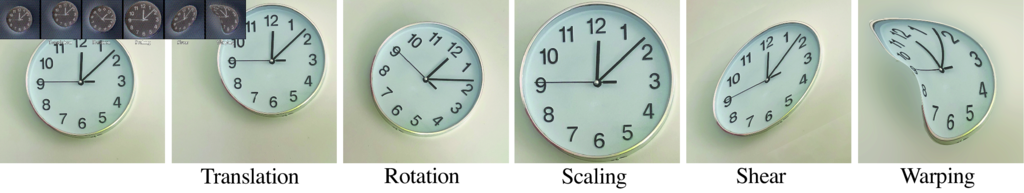
\includegraphics[width=1\linewidth]{figures/imaging_geometry/2d_transformations.eps}
}
\caption{2D geometric transformations. 
%On the left we see the original image. The next four transformations correspond to translation, rotation, scaling and shear. Those four transformations can be easily described with matrices. 
The final transformation is an arbitrary warping with a more complex deformation field.}
\label{fig:2dtransformations_clock}
\end{figure}

%\subsection{Translation, Rotation, Scaling and Shear.}

We'll explore the use of homogeneous coordinates for describing 2D geometric transformations first, then see how they can easily represent 3D perspective projection.


\subsection{Translation}

Consider a translation by a 2D vector, $(t_x, t_y)$ as shown in \fig{\ref{fig:translations}}. We'll denote the coordinates after the transformation with a prime. In heterogeneous coordinates, we have
\begin{equation}
    \begin{pmatrix}
    x' \\
    y' 
    \end{pmatrix}
    =
    \begin{pmatrix}
    x \\
    y 
    \end{pmatrix}
    +
    \begin{pmatrix}
    t_x \\
    t_y 
    \end{pmatrix}
\end{equation}
We can write this translation in homogeneous coordinates by the product:
\begin{equation}
    \begin{bmatrix}
    x' \\
    y' \\
    1
    \end{bmatrix}
    =
    \begin{bmatrix}
    1 & 0 & t_x \\
    0 & 1 & t_y \\
    0 & 0 & 1
    \end{bmatrix}
    \begin{bmatrix}
    x \\
    y \\
    1
    \end{bmatrix}
\end{equation}
What is interesting is that we have transformed an addition into a product by a matrix, $\mathbf{T}$, and a vector, $\mathbf{p}$, in homogeneous coordinates. 
Rewriting the equation above as:
\begin{equation}
    \mathbf{p}' = \mathbf{T} \mathbf{p},
\end{equation}
with the homogeneous matrix, $\mathbf{T}$, defined as
\begin{equation}
    \mathbf{T} =             
    \begin{bmatrix}
    1 & 0 & t_x \\
    0 & 1 & t_y \\
    0 & 0 & 1
    \end{bmatrix}
\end{equation}
For calculations in homogeneous coordinates, both matrices and vectors are only defined up to an arbitrary (non-zero) multiplicative scaling factor.

To cascade two translation operations $\mathbf{t}$ and  $\mathbf{s} $, in heterogeneous coordinates, we have 
\begin{equation}
     \mathbf{p}' = \mathbf{p} + \mathbf{t}  + \mathbf{s}   
\end{equation}


\begin{figure}[ht]
\centerline{
\includegraphics[width=.7\linewidth]{figures/imaging_geometry/translations.eps}
}
\caption{(left) Translation. (right) Composition of two consecutive translations.}
\label{fig:translations}
\end{figure}


In homogeneous coordinates, we cascade the corresponding translation matrices:
\begin{equation}
     \mathbf{p}' = \mathbf{S} \mathbf{T} \mathbf{p},
\end{equation}
where the homogeneous translation matrix, $\mathbf{S}$, corresponding to the offset $\mathbf{s}$, is:
\begin{equation}
    \mathbf{S} =            
    \begin{bmatrix}
    1 & 0 & s_x \\
    0 & 1 & s_y \\
    0 & 0 & 1
    \end{bmatrix}
\end{equation}

You can check that:
\begin{equation}
    \begin{bmatrix}
    1 & 0 & t_x \\
    0 & 1 & t_y \\
    0 & 0 & 1
    \end{bmatrix}
    \begin{bmatrix}
    1 & 0 & s_x \\
    0 & 1 & s_y \\
    0 & 0 & 1
    \end{bmatrix}
    =
    \begin{bmatrix}
    1 & 0 & t_x+s_x \\
    0 & 1 & t_y+s_y \\
    0 & 0 & 1
    \end{bmatrix}
\end{equation}

In summary, in homogeneous coordinates a translation becomes a product with a matrix, and chaining translations can be done by multiplying the matrices together. The benefits of using the homogeneous coordinates will become more obvious later.

\subsection{Scaling}

Scaling the $x$-axis by $s_x$ and the $y$-axis by $s_y$, shown in \fig{\ref{fig:scaling}}, yields the transformation matrix in homogeneous coordinates,
\begin{equation}
    \mathbf{S} =             
    \begin{bmatrix}
    s_x & 0 & 0 \\
    0 & s_y & 0 \\
    0 & 0 & 1
    \end{bmatrix}
\end{equation}

The scaling matrix is a diagonal matrix. 

\begin{figure}[ht]
\centerline{
\includegraphics[width=.6\linewidth]{figures/imaging_geometry/scaling.eps}
}
\caption{Non-uniform or anisotropic scaling. In this example the $y$-axis is compressed and the $x$-axis is expanded.}
\label{fig:scaling}
\end{figure}

Uniform scaling is obtained when $s_x=s_y$, otherwise the scaling is nonuniform or anisotropic. After uniform scaling, all of the angles are preserved. In all cases, parallel lines remain parallel. Areas are scaled by the determinant of the scaling matrix.


\subsection{Rotation}

For a rotation by an angle $\theta$, \fig{\ref{fig:rotation}}, we simply have the matrix in homogeneous coordinates:
\begin{equation}
    \mathbf{R} =             
    \begin{bmatrix}
    \cos(\theta) & \sin(\theta) & 0 \\
    -\sin(\theta) & \cos(\theta) & 0 \\
    0 & 0 & 1
    \end{bmatrix}
\end{equation}


\begin{figure}
\centerline{
\includegraphics[width=.6\linewidth]{figures/imaging_geometry/rotation.eps}
}
\caption{Rotation by an angle $\theta$ counterclockwise around the origin.}
\label{fig:rotation}
\end{figure}


As in the case of the translation, a rotation in homogeneous coordinates is a product
\begin{equation}
    \mathbf{p}' = \mathbf{R} \mathbf{p},
\end{equation}
Also, as we should expect, chaining two rotations with angles $\alpha$ and $\beta$, is the same than applying a rotation with an angle $\alpha+\beta$. You can check that multiplying the two rotation matrices you get the right transformation. 

The determinant of a rotation matrix is 1 and the matrix is orthogonal, that is the transpose is equal to the inverse: $\mathbf{R}^\transpose = \mathbf{R}^{-1}$. The inverse is also a rotation matrix. The distance between any point and the origin does not change after a rotation. 

In heterogeneous coordinates, the transformation can also be written in the same way but using only the upper-left $2\times2$ matrix. Representing rotations in homogeneous coordinates has no benefit with respect to heterogeneous coordinates. But the advantage is that now both rotation and translation are written in the same way! They are both products of a matrix times a vector, so that they can be combined as we will discuss in \sect{\ref{sec:chaining_transformations}}.   


If the angle of rotation is very small, then we can approximate the rotation matrix by its Taylor development
(for small $x$, $\sin(x) \approx x$ and $\cos(x) \approx 1$):
\begin{equation}
    \mathbf{R} \simeq            
    \begin{bmatrix}
    1 & \theta & 0 \\
    -\theta & 1 & 0 \\
    0 & 0 & 1
    \end{bmatrix}
\end{equation}

For small angles a rotation becomes a shear, which we will discuss next. In general, for all angles, a rotation can be written as two shears and a scaling.

Rotations in 3D become more complex as there are multiple possible parametrizations. 


\subsection{Shearing}

Shearing involves scale factors in the off-diagonal matrix locations, as shown in the matrix, $\mathbf{Q}$:
\begin{equation}
    \mathbf{Q} =             
    \begin{bmatrix}
    1 & q_x & 0 \\
    q_y & 1 & 0 \\
    0 & 0 & 1
    \end{bmatrix}
\end{equation}

\Fig{\ref{fig:shear}} shows examples with an horizontal shear ($qx=1, q_y=0$), a vertical shear ($q_x=0, q_y=1$), and an arbitrary shear. 

\begin{figure}
\centerline{
\includegraphics[width=1\linewidth]{figures/imaging_geometry/shear.eps}
}
\caption{Three examples of shear transformation.}
\label{fig:shear}
\end{figure}

In the example of the horizontal shear, the points are displaced along horizontal lines by displacement proportional to the $y$ coordinate, $x'=x+q_y y$. 

In a shear, lines are mapped to lines, parallel lines remain parallel, (non-zero) angles between lines change.

\subsection{Chaining Transformations}
\label{sec:chaining_transformations}

As we have seen, homogeneous coordinates allows using all the four different transformations as matrix multiplications. We can now build complex transformations by combining these four transformations:
\begin{equation}
    \mathbf{p}' = 
    \begin{bmatrix}
    1 & q_x & 0 \\
    q_y & 1 & 0 \\
    0 & 0 & 1
    \end{bmatrix}
    \begin{bmatrix}
    s_x & 0 & 0 \\
    0 & s_y & 0 \\
    0 & 0 & 1
    \end{bmatrix}
    \begin{bmatrix}
    \cos(\theta) & \sin(\theta) & 0 \\
    -\sin(\theta) & \cos(\theta) & 0 \\
    0 & 0 & 1
    \end{bmatrix}
    \begin{bmatrix}
    1 & 0 & t_x \\
    0 & 1 & t_y \\
    0 & 0 & 1
    \end{bmatrix}
    \mathbf{p}
\end{equation}

%\begin{equation}
%    \mathbf{p}' = 
%    \mathbf{M}  
%    \mathbf{p}
%\end{equation}

 In heterogeneous coordinates the translation will have to be modeled as an addition breaking the homogeneity of this equation. The transformations described in this section are summarized in \fig{\ref{fig:2dtransformations}}.

\begin{figure}
\centerline{
\includegraphics[width=1\linewidth]{figures/imaging_geometry/2d_transforms.eps}
}
\caption{Summary of 2D geometric transformations and their formulation in homogeneous coordinates.}
\label{fig:2dtransformations}
\end{figure}


As matrix operation are noncommutative, the order in which operations are done is important (i.e., it is not the same to rotate with respect to the origin and then translate, as it is to translate and then rotate). All of the geometric transformations we have described are relative to the origin. If you want to rotate an image around an arbitrary central location, then you need to first translate to put that location at the origin, then rotate and then translate back. 

\begin{equation}
    \mathbf{p}' = 
    \begin{bmatrix}
    1 & 0 & t_x \\
    0 & 1 & t_y \\
    0 & 0 & 1
    \end{bmatrix}
    \begin{bmatrix}
    \cos(\theta) & \sin(\theta) & 0 \\
    -\sin(\theta) & \cos(\theta) & 0 \\
    0 & 0 & 1
    \end{bmatrix}
    \begin{bmatrix}
    1 & 0 & -t_x \\
    0 & 1 & -t_y \\
    0 & 0 & 1
    \end{bmatrix}
    \mathbf{p}
\end{equation}

Chaining transformations in such a way is a very important tool in computer graphics and we will also use it extensively as we dive deeper into geometry. 

When chaining rotations and translations only we will have a {\bf euclidean transformation} 
\index{Euclidean transformation}
(lengths and angles between lines are preserved). A {\bf similarity transform}
\index{Similarity transform}
is the result of chaining a rotation, translation and scaling (with uniform scaling, $s_x=s_y$). In this case angles are preserved but not lengths. Chaining all transformations results in an {\bf affine transformation}. 
\index{Affine transformation}
Each set of transformations forms a group.  

\subsection{Generic 2D Transformations}

In general, chaining translations, scalings, rotations and shears will result in a generic matrix with the form:
\begin{equation}
    \mathbf{p}' = 
    \begin{bmatrix}
    a & b & c \\
    d & e & f \\
    0 & 0 & 1
    \end{bmatrix}
    \mathbf{p}
\end{equation}
Any transformation with that form (6 degrees of freedom) is an affine transformation. An affine transformation has the property that parallel lines will remain parallel after the transformation; however, lengths and non-zero angles might change. 

As the last row of the transformation is $[0,0,1]$, one could be tempted to drop it and go directly from homogeneous to heterogeneous, using the top $2 \times 3$ matrix, but this will only work if the input vector has a 1 in the third component. 

What happens if we have 9 degrees of freedom?

\begin{equation}
    \mathbf{p}' = 
    \begin{bmatrix}
    a & b & c \\
    d & e & f \\
    g & h & i
    \end{bmatrix}
    \mathbf{p}
\end{equation}
In fact we only have 8 degrees of freedom as a global scaling of the matrix does not change the homogeneous coordinates. The set of transformations described by this full matrix becomes more general than the transformations described in the previous sections. The additional degrees of freedom include {\bf elations} and {\bf projective transformations}. 
\index{Projective transformation}

\subsection{Geometric Transformations as Convolutions}

In \chap{\ref{chapter:linear_image_filtering}} we showed how certain geometric transformations can be written as convolutions (such as the translation) while others cannot (such as rotations, scalings, shears, etc.). However, things change when adding geometry explicitly to the image representation! 

Once geometry is added to the representation, all of the transformations we discussed before can be implemented as one-dimensional (1D) convolutions over the locations as shown in the diagram in \fig{\ref{fig:rotation_as_convolution}}. 


\begin{figure}[ht]
\centerline{
\includegraphics[width=.6\linewidth]{figures/imaging_geometry/rotation_as_convolution.eps}
}
\caption{Geometric transformation as a convolution. The input and output signals are represented as pixel sets with explicit geometry. The convolution kernels are $w_x$ and $w_y$, corresponding to one dimensional convolutions as they only mix input features within the same input vector. The output intensity values are the same as the input.}
\label{fig:rotation_as_convolution}
\end{figure}

In the diagram (\fig{\ref{fig:rotation_as_convolution}}), each input element is a vector
$(x_i,y_i,\img_i)$
where $x_i$, $y_i$ are the pixel location, and $\img_i$ is the pixel intensity at that location. 
The convolution kernels are: $w_x=[\cos ( \theta), \sin ( \theta)]$ and  $w_y=[-\sin ( \theta), \cos ( \theta)]$. The weights are the same for all inputs. The output is also represented using position explicitly: $(x'_i,y'_i,\img'_i)$.


However, note that to perform a convolution on the output intensity will require translating the position encoding back into an image on a rectangular grid. For instance, after a rotation, the locations for the intensity values will change and the pixels will not lie on a rectangular grid anymore. The convolution kernels for the intensity channel will have to be transformed too.

\section{Lines and Planes in Homogeneous Coordinates}

One interesting application of homogeneous coordinates is to use it to describe lines and planes and perform operations with them. In 2D, the equation of a line is $ax+by+c=0$, which can be written in homogeneous coordinates as
\begin{equation}
    ax+by+c=0 \rightarrow 
    \begin{bmatrix}
    a & b & c 
    \end{bmatrix}
    \begin{bmatrix}
    x \\
    y \\
    1
    \end{bmatrix}
    = 0
\end{equation}

In homogeneous coordinates, the equation of a line is the dot product:
\begin{equation}
    \boldsymbol{l} ^\transpose \mathbf{p} = 0
\end{equation}
where $\boldsymbol{l}^\transpose = \left [a, b, c\right ]$. Therefore, a point $\mathbf{p}$, belongs to the line when $\boldsymbol{l}$ and $\mathbf{p}$ are perpendicular. 


This representation of the line is in homogeneous coordinates because it is scale invariant. This is, $\left [a, b, c\right ]$ is the same line as $\left [a/c, b/c, 1\right ]$. Therefore, it is also useful to describe the equation of the line with $\boldsymbol{l}^\transpose = \left [n_x, n_y, -d\right ]$ where $(n_x,n_y)$ is the normal to the line and $d$ is the distance to the origin. 

Using homogeneous coordinates makes obtaining geometric properties of points and lines very easy. Given two points $\mathbf{p}_1$ and $\mathbf{p}_2$ in homogeneous coordinates, the line that passes by both points is the cross product (\fig{\ref{fig:points_and_lines_homogeneous_imggeo}}):
\begin{equation}
    \boldsymbol{l} = \mathbf{p}_1 \times \mathbf{p}_2
\end{equation}
This is because if the line passes by both points, it has to verify that $\boldsymbol{l}^\transpose \mathbf{p}_1=0$ and  $\boldsymbol{l}^\transpose \mathbf{p}_2=0$. That is, the vector $\mathbf{l}$ has to be perpendicular to both $\mathbf{p}_1$ and $\mathbf{p}_2$. The cross product between $\mathbf{p}_1$ and $\mathbf{p}_2$ gives a vector that is perpendicular to both.

Following a similar argument, you can show that given two lines $\boldsymbol{l}_1$ and $\boldsymbol{l}_2$ the intersection point between them is the cross product (\fig{\ref{fig:points_and_lines_homogeneous_imggeo}}):
\begin{equation}
    \mathbf{p} = \boldsymbol{l}_1 \times  \boldsymbol{l}_2
\end{equation}
The coordinates of $\mathbf{p}$ computed that way will be given in homogeneous coordinates. So you need to divide by the third component in order to get the actual point coordinates in heterogeneous coordinates. 

\begin{figure}[t]
\centerline{
%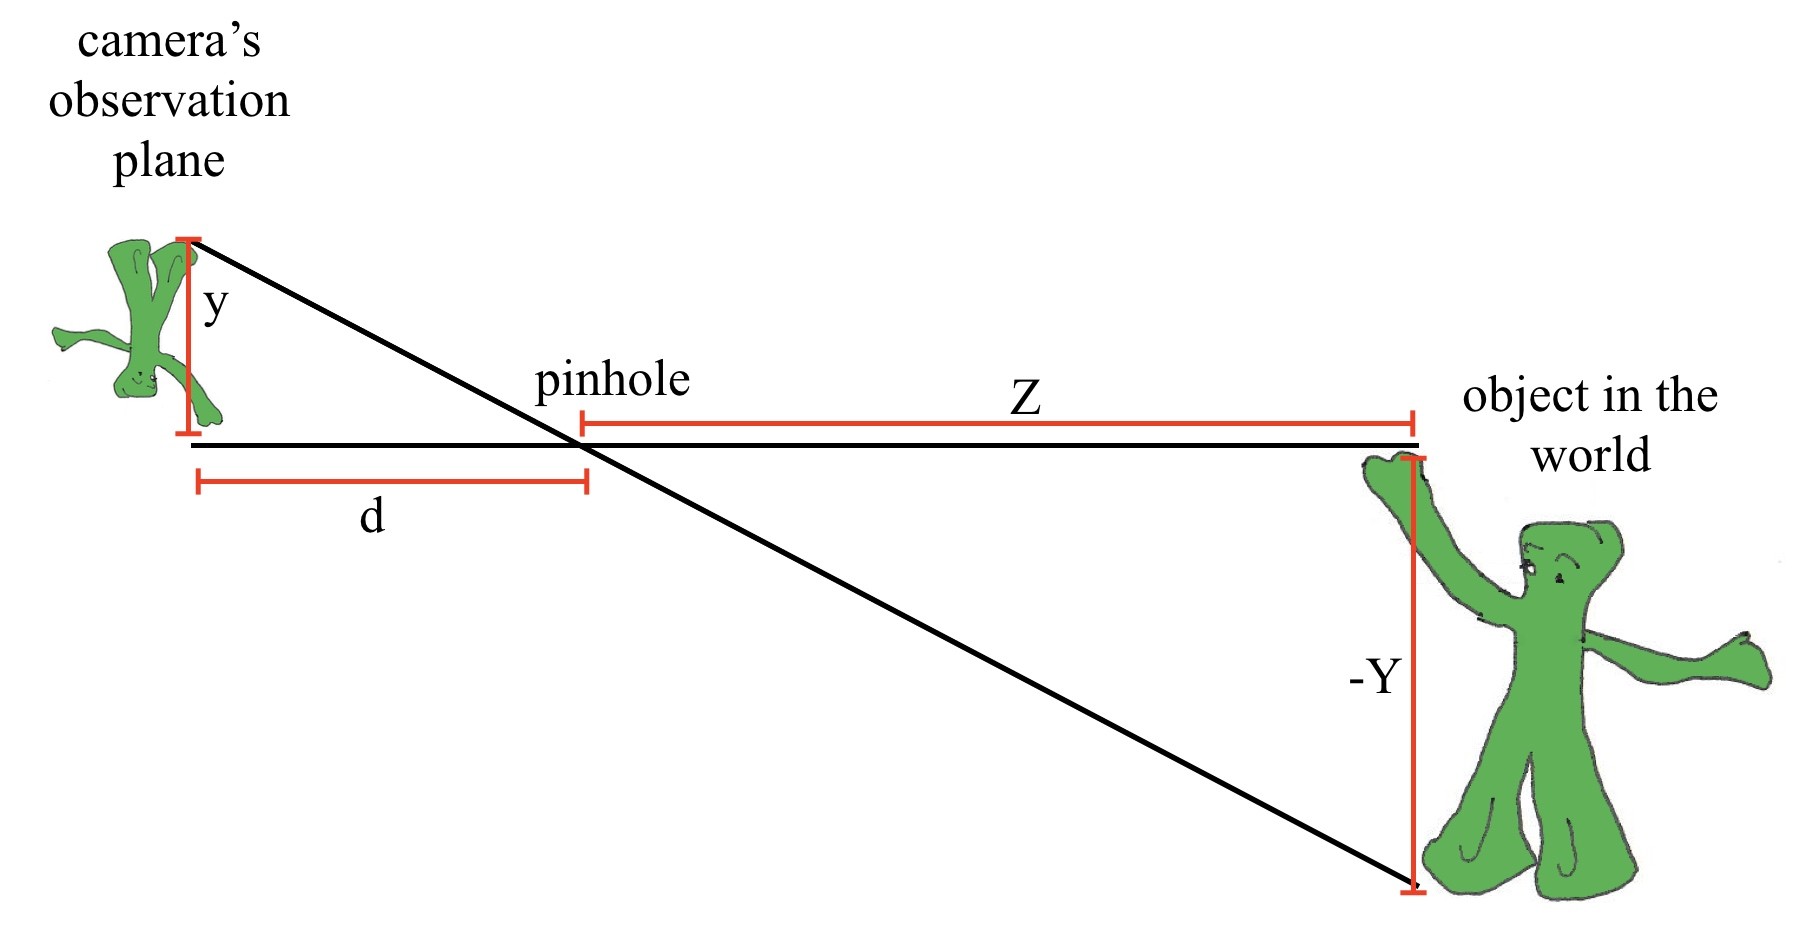
\includegraphics[width=.8\linewidth]{figures/imaging/pinholeGeomGumby.jpg}
\includegraphics[width=.7\linewidth]{figures/imaging_geometry/points_and_lines_homogeneous.eps}
}
\caption{Using homogeneous coordinates to get the line that passes by two points, and to obtain the intersection of two lines. Both operations are analogous.}
\label{fig:points_and_lines_homogeneous_imggeo}
\end{figure}

If three 2D points are colinear, then the determinant of the matrix formed by concatenating the three vectors, in homogeneous coordinates, as columns is equal to zero: $\det( [\mathbf{p}_1~\mathbf{p}_2~\mathbf{p}_3 ])=0$. If three lines intersect in the same point we have a similar relationship: $\det( [\boldsymbol{l}_1~\boldsymbol{l}_2~\boldsymbol{l}_3 ])=0$.

It is also interesting to point out that a 3D vector can be interpreted as a 2D line or as a 2D point in homogeneous coordinates. 

We can also do something analogous to represent planes in 3D. The equation of a 3D plane is $aX+bY+cZ+d=0$, which can be written in homogeneous coordinates as:

\begin{equation}
    \mathbf{\pi}^\transpose   \mathbf{P} = 0
\end{equation}
where $\mathbf{\pi} = [a,b,c,d]^\transpose$ are the plane parameters and $\mathbf{P}=[X,Y,Z,1]^\transpose$ are the 3D point homogeneous coordinates. 





Representing 3D lines with homogeneous coordinates is not that easy and the reader can consult other sources \cite{Hartley2004} to learn more about representing geometric objects in homogeneous coordinates.

\section{Image Warping}
\label{sect:image_warping}

Now that we have seen how to describe simple geometric transformations to  pixel coordinates, we need to go back to the representation of the image as samples on a regular grid. This will require applying image interpolation.

The first algorithm that usually comes to mind when transforming an image is to take every pixel in the original image represented as $[\img_i,x_i,y_i]$, apply the transformation, $\mathbf{M}$, to the coordinates, and record the pixel color into the resulting coordinates in the target image (\fig{\ref{fig:warping_sketch}}). As coordinates might result in non-integer values, we can simply round the result to the closest pixel coordinate (i.e., nearest neighbor interpolation as we discussed in \sect{\ref{sec:interpolation}}). This algorithm is called {\bf forward mapping}.
\index{Forward mapping}
It is an intuitive way of warping an image but it is really not a good idea. We will have all sorts of artifacts such as missing values and aliasing as shown in figures \ref{fig:warping_sketch} and \ref{fig:warping_forward_backward}.


\begin{figure}[t]
\centerline{
%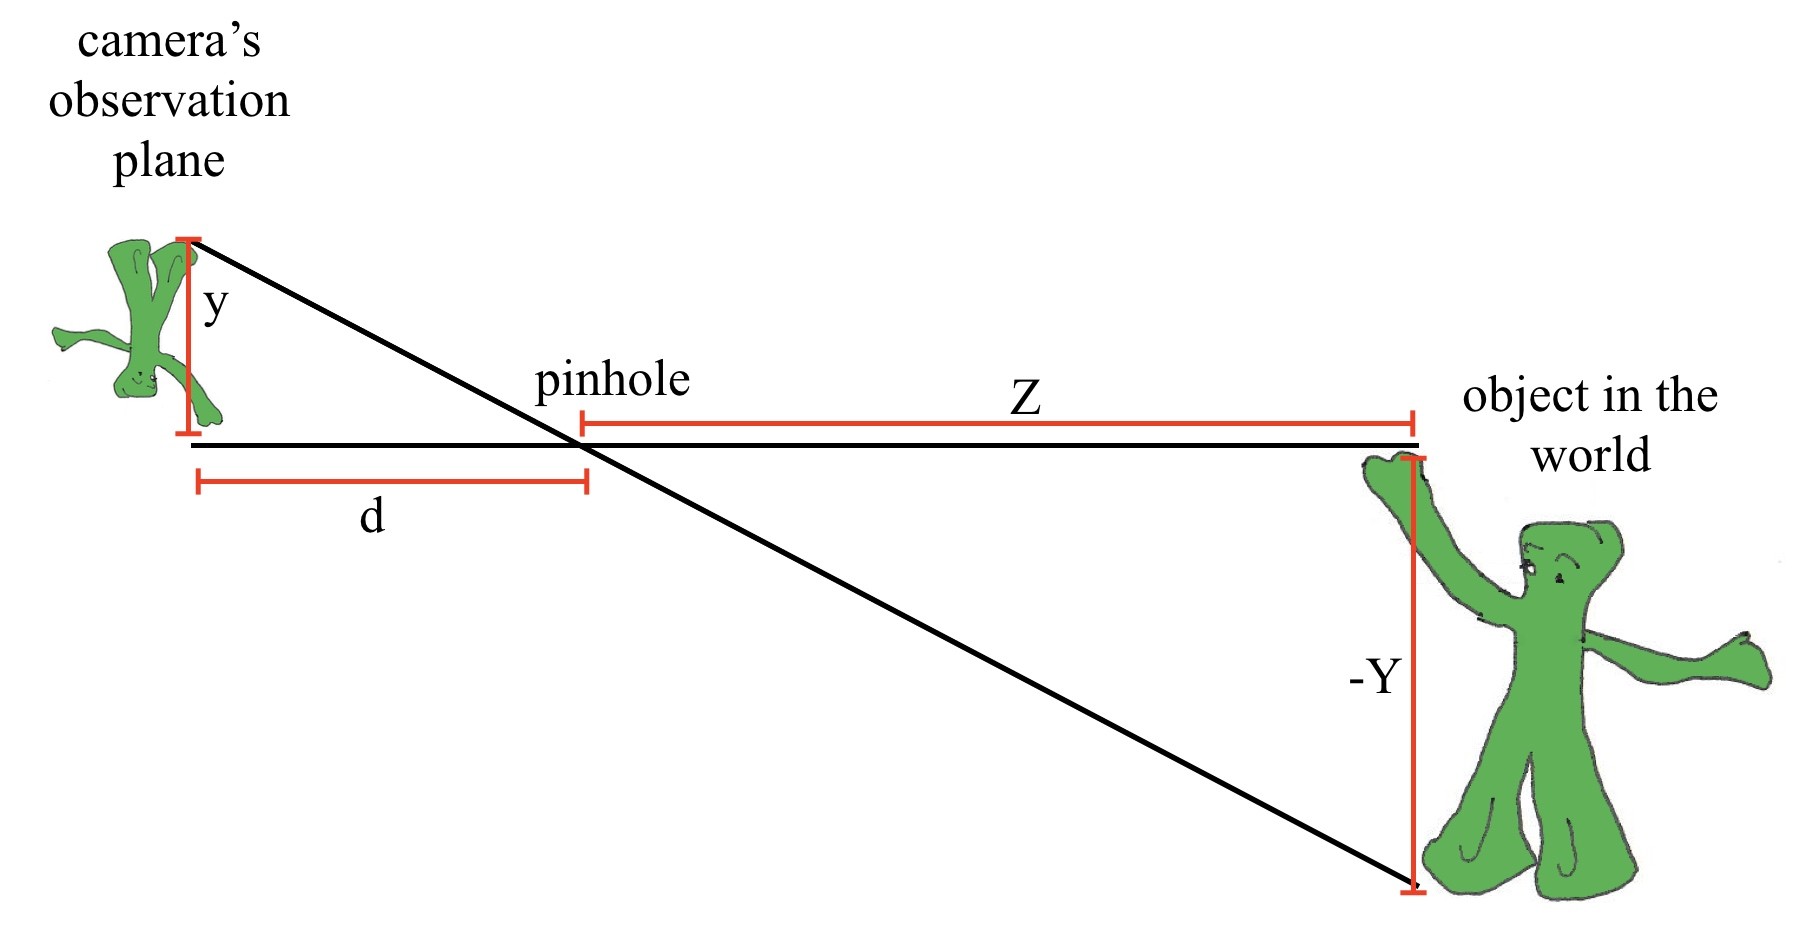
\includegraphics[width=.8\linewidth]{figures/imaging/pinholeGeomGumby.jpg}
\includegraphics[width=1\linewidth]{figures/imaging_geometry/warping_sketch.eps}
}
\caption{Comparison between forward and backward mapping using nearest neighbor interpolation. Forward mapping will produce missing values.}
\label{fig:warping_sketch}
\end{figure}


The best approach is to use what is called {\bf backward mapping} 
\index{Backward mapping}
which consists of looping over all the pixels of the target image and applying the inverse geometric transform, $\mathbf{M}^{-1}$; we then use interpolation (as described in \sect{\ref{sec:interpolation}} in \chap{\ref{chap:downsampling_and_upsampling}}) to get the correct color value (\fig{\ref{fig:warping_sketch}}). This process guarantees that there will be no missing values (unless the coordinates go outside the frame of the input image) and there will be no aliasing if the interpolation is done correctly. To avoid aliasing, blurring of the input image might be necessary if the density of pixels in the target image is lower than in the input image. Figures \ref{fig:warping_sketch} and \ref{fig:warping_forward_backward} compare forward and backward mapping. 


\begin{figure}[t]
\centerline{
%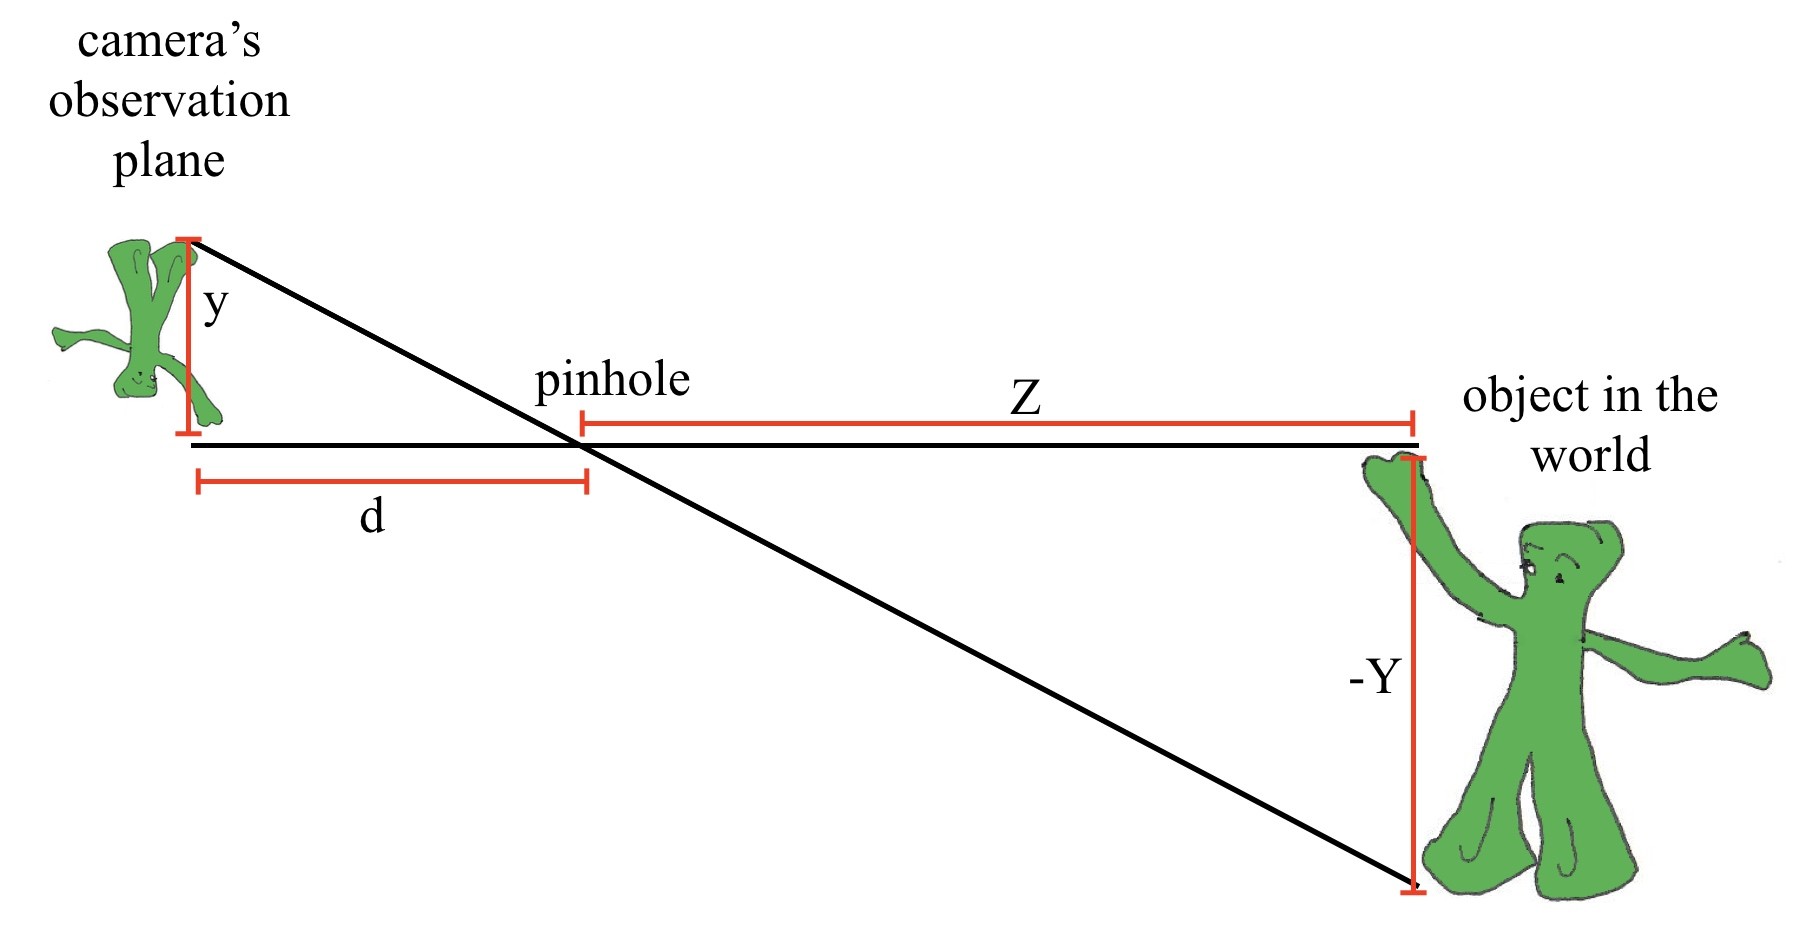
\includegraphics[width=.8\linewidth]{figures/imaging/pinholeGeomGumby.jpg}
\includegraphics[width=1\linewidth]{figures/imaging_geometry/warping_forward_backward.eps}
}
\caption{Comparison between forward and backward mapping. Forward mapping produces many artifacts. In both cases we use nearest neighbor interpolation.}
\label{fig:warping_forward_backward}
\end{figure}


To achieve high image quality warping it is important to chose a high quality interpolation filter such as bilinear, bicubic, or Lanczos. MIP-mapping \cite{Lance1983} is another popular technique for high quality and efficient interpolation. MIP-mapping relies on a multiscale image pyramid to efficiently compute the best neighborhood structure needed to perform the interpolation at each location, which can be very useful when warping an image onto a curved surface. 
\index{MIP-mapping}
%\marginnote{An implicit }

Image warping can be applied to arbitrary geometric transformations and not just the ones described in this section. 




%\begin{algorithm}[h]
%\label{alg:warping}
%\SetAlgoVlined
%\DontPrintSemicolon
%\caption{Image warping}
%{\bf Input:} Image: $\mathbf{s} \in \mathbb{R}^{N \times M \times 3}$, location: $\mathbf{p} = (x,y)^T$
%{\bf Output:} Interpolated sample $\hat{s}$;
%{\bf Parameters:} geometric transformation: $\mathbf{M}^{-1}$, $method$ = type of interpolation\;
%{\bf Compute:} $\mathbf{p}' = \mathbf{M}^{-1}\mathbf{p}$\;
%{\bf Compute:} $\hat{s} = Interpolate (\mathbf{s}, \mathbf{p}', method)$\;
%\For{\upshape $i = 0, \dots, M-1$} 
%{
%\For{\upshape $j = 0, \dots, N-1$}
%{
%    $u[i,j], v[i,j] = inv(\mathbf{A} [i,j])  \textbf{b}[i,j] $\;
%}
%}
%\end{algorithm}


%\subsection{Warping with implicit image representations}
\section{Implicit Image Representations}\label{sec:implicit_image_representations}

An image is an array of values, $\boldimg \in \mathbb{R}^{N \times M \times 3}$, where each value is indexed as $\img [n,m]$ when $n,m$ take only on discrete values. We can say that interpolation is a way of transforming the discrete image into a continuous signal: $\img (x,y)$.

An implicit image representation via a function $f_\theta$ trained to reproduce the image pixels is a function such that,
\begin{equation}
   \img (x,y) = f_{\theta}(x,y)
\end{equation}
where now $x,y$ can take on any real value. 
\marginnote{An image represented using a neural network: 
\\[6pt]
\includegraphics[width=1\linewidth]{figures/imaging_geometry/xy_mlp_rgb.eps}
\\[6pt]
Once the network is trained to reproduce the image pixel colors for each input location, the parameters of the network correspond to a compressed representation of the original image. 

For this representation to work better, the input location is usually first transformed using {\bf positional encoding}, and the final network is more complex than the one shown here. We will discuss this type of representations more in depth in \chap{\ref{chapter:nerfs}}.
}

\subsection{Interpolation}

In the case of nearest neighbors or bilinear interpolation, the parameters of the interpolation function $\theta$ is the input image itself. For example, using a functional form, nearest neighbors interpolation can be written as:
\begin{equation}
   \img (x,y) = \img \left[ \text{round}(x), \text{round}(y) \right]
\end{equation}

What is really interesting about thinking about interpolation in this way is that we can now extend the space of possible functions $f_{\theta}(x,y)$ to include other functional forms. For instance, this function could be implemented by a neural network that will take as input the two image coordinate values $x$ and $y$ and will output the intensity value at that location. The training set for the neural network is the image itself, and it will consist of the input-output pairs $[(x_i, y_i); \img(x_i,y_i)]$ (i.e., location as input and intensities/colors as output). During training the neural network will memorize the image. The training will contain only values at discrete positions but in test time we can use any continuous input values. For this formulation to work, the neural network should be able to generalize to non-integer coordinate values, that is, it should be able to interpolate between samples. 

\subsection{Image Warping with Implicit Representations}

Once the neural network, $f_{\theta}(x,y)$, has learned to reproduce the image, we can reconstruct the original image or apply transformations to it. Image warping is then implemented by simply applying the inverse geometric transformation to the discrete coordinates of the output grid and use the functional representation of the image to get the interpolated values:
\begin{equation}
   \hat{\img} (x,y) = f_{\theta} \left( \mathbf{M}^{-1}(x,y,1)^\transpose \right)
\end{equation}
In this equation the input location is written in homogeneous coordinates, so the function $f$ will first have to divide by the third component to translate the input back to heterogeneous coordinates. 
% Cameraman picture is available here:
% https://imageprocessingplace.com/root_files_V3/image_databases.htm
% https://dome.mit.edu/handle/1721.3/195767

The example in \fig{\ref{fig:siren_rotation_and_scaling}} shows an image encoded by a sinusoidal representation network (SIREN) \cite{sitzmann2019siren} and then 
reconstructed with a rotation of 45 degrees and a scaling by 0.5 along both dimensions. 

\begin{figure}[t]
\centerline{
%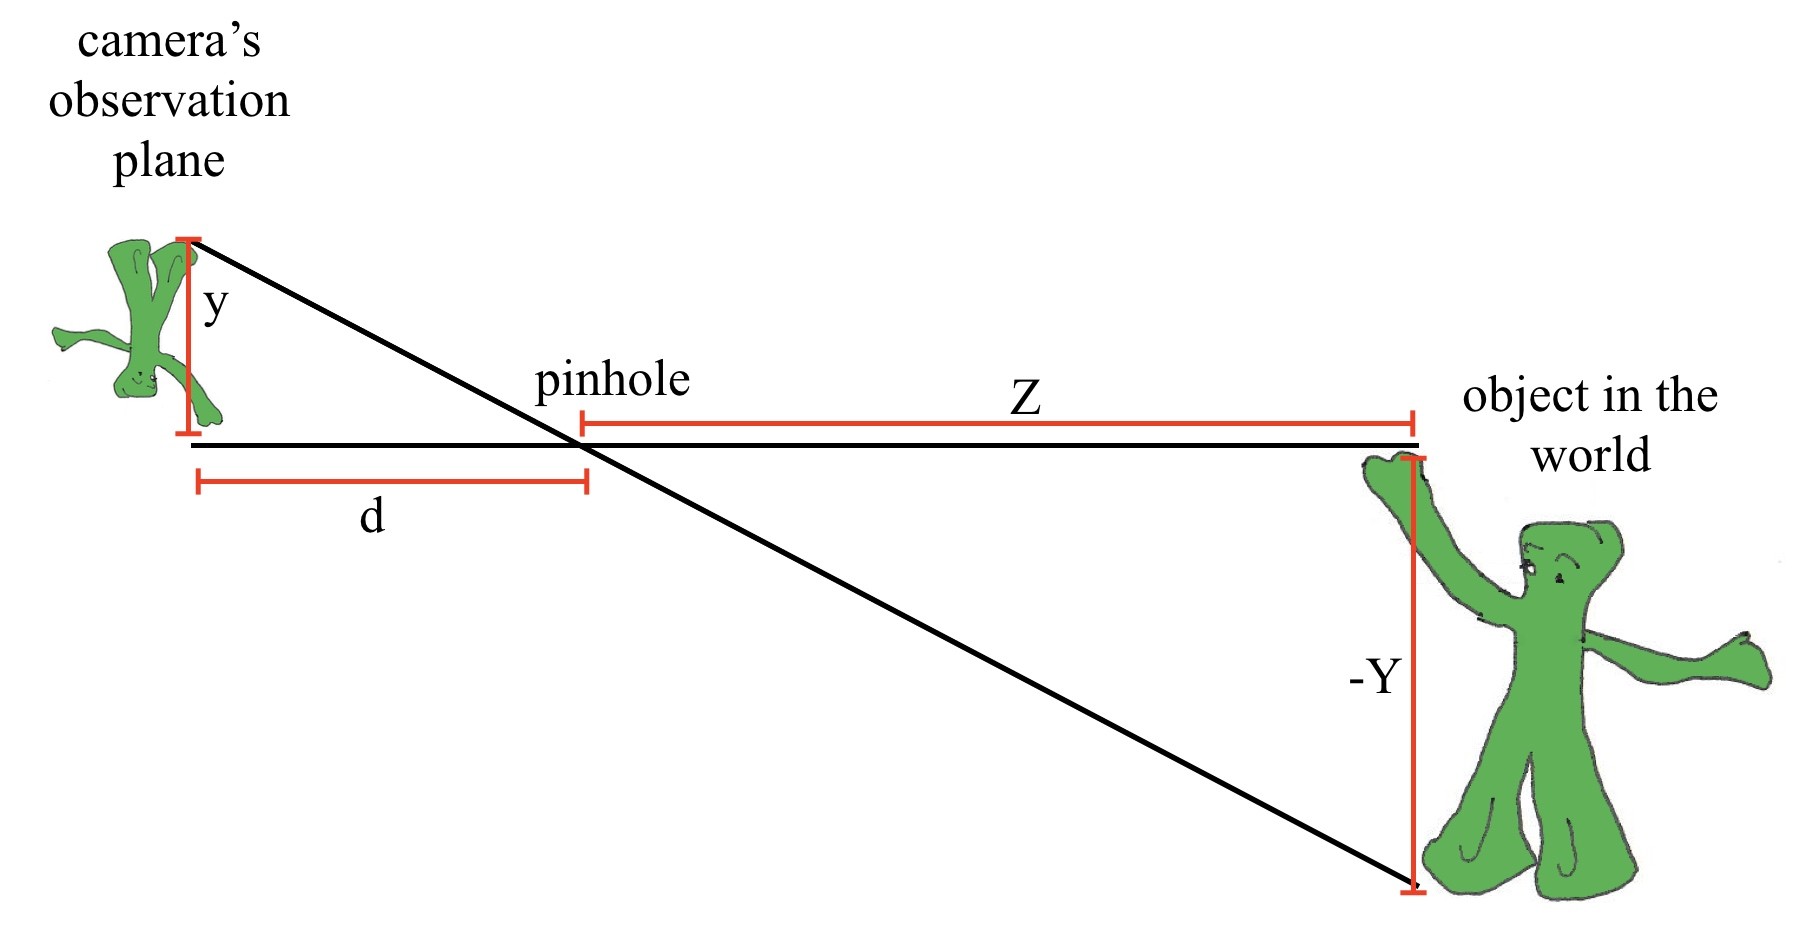
\includegraphics[width=.8\linewidth]{figures/imaging/pinholeGeomGumby.jpg}
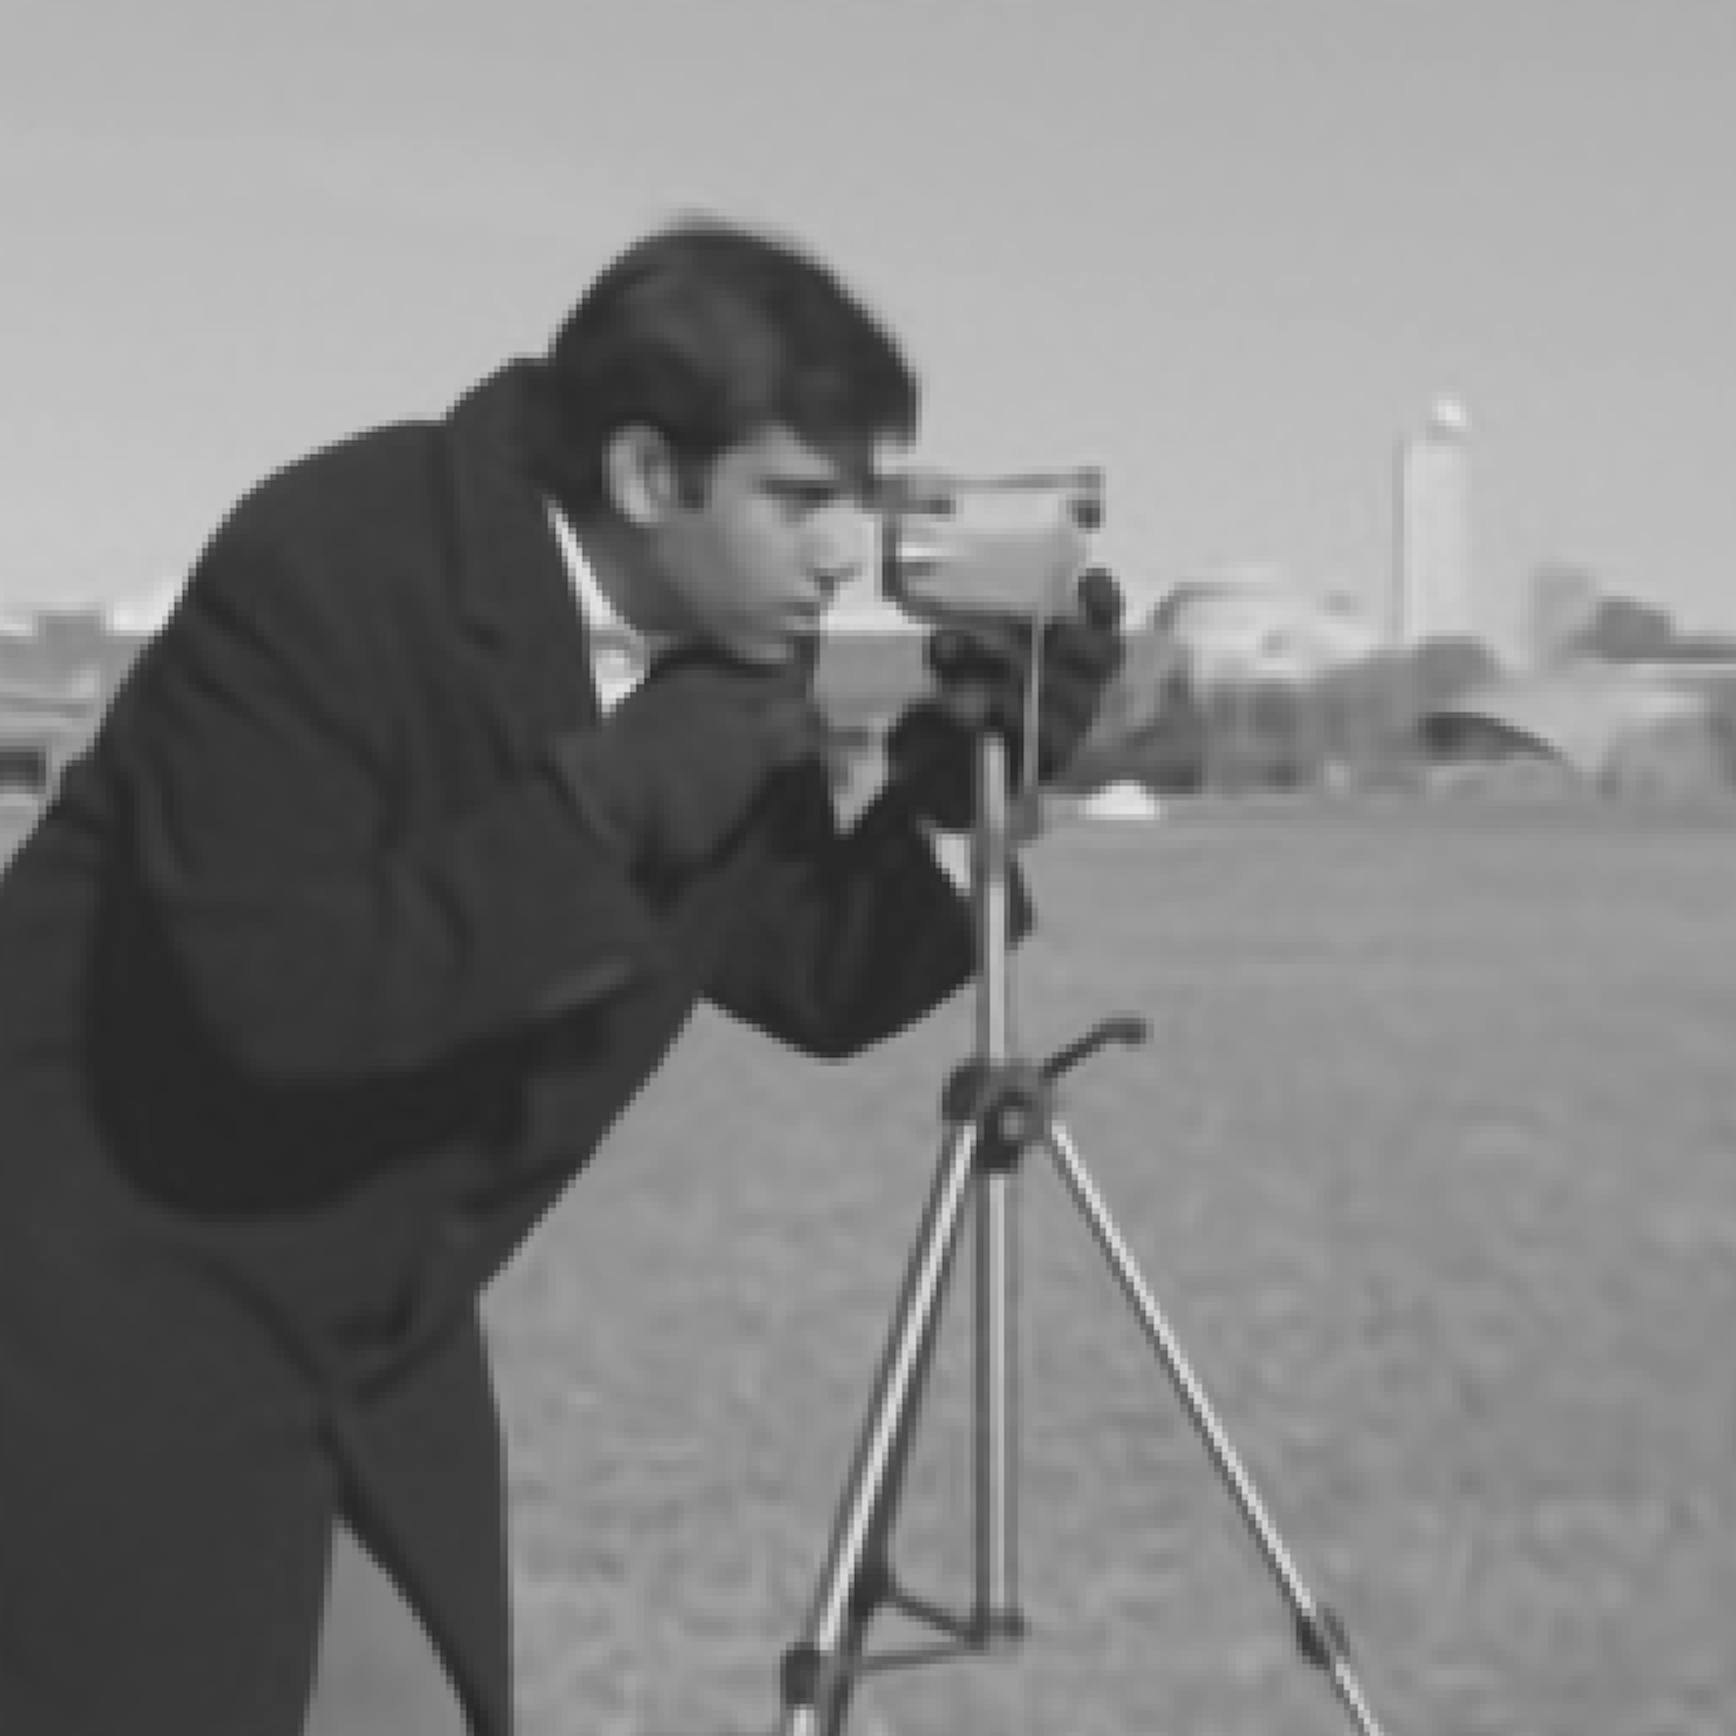
\includegraphics[width=.49\linewidth]{figures/imaging_geometry/siren_original_image.png}
~
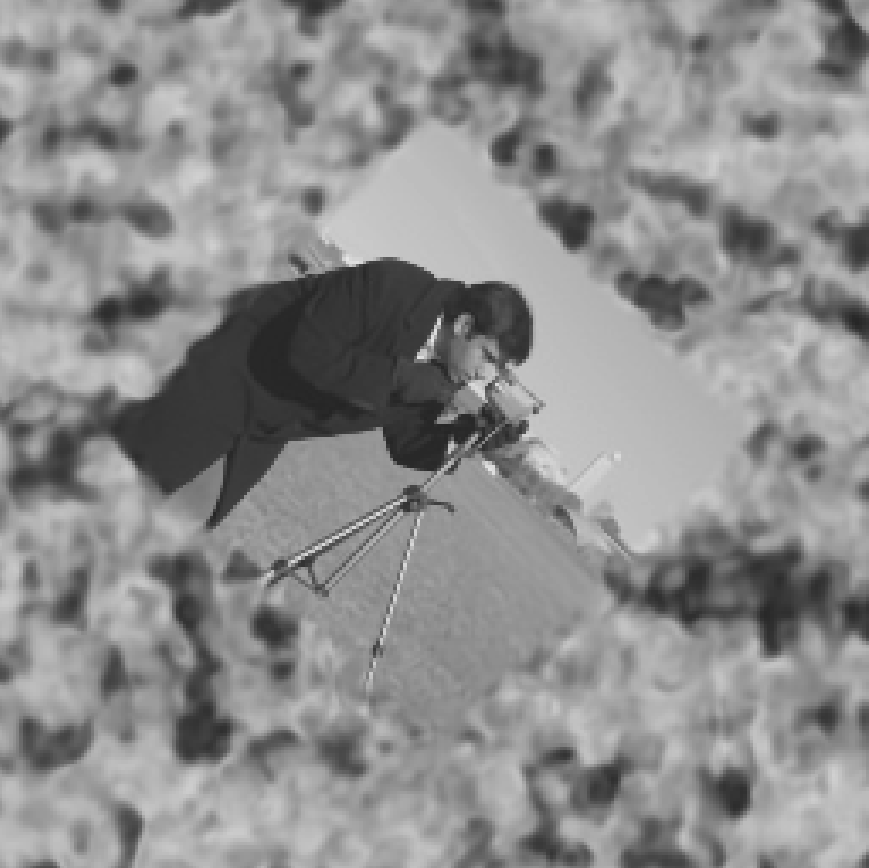
\includegraphics[width=.49\linewidth]{figures/imaging_geometry/siren_rotation_and_scaling.png}
}
\caption{(left) Image encoded by SIREN. (right) Image reconstructed with a rotation of 45 degrees and a scaling by 0.5 along both dimensions.}
%\caption{Comparison between forward and backward mapping. Forward mapping produces many artifacts. In both cases we use nearest neighbor interpolation.}
\label{fig:siren_rotation_and_scaling}
\end{figure}

%\marginnote{The {\bf cameraman} picture, taken at MIT around 1978, became a popular image in image processing. We can see the MIT dome and building 54 on the background.}
From this result we can make a few observations. First, we can see that, due to the transformation, there is aliasing in the sampled image (aliasing is most visible in the leg of the tripod). One way of avoiding aliasing would be by sampling the output on a finer grid and then blurring and downsampling the result to the desired image size.
The second observation is that the way the boundary is extended is not like any of the methods that we studied in chapter \ref{chapter:linear_image_filtering}; instead the image is padded by some form of noise that smoothly extends the image without adding strong image derivatives.

%the interpolation is not one of the standard interpolations we have seen before. But it is translational invariant, it is just not a linear function. 

%\subsection{Image Alignment}

We can also study the reverse problem where we have two images (one is a transformed version of the other) and the goal is to identify the transformation $\mathbf{M}$. This problem is called {\bf image alignment}.



The spatial transformer network \cite{Jaderberg2015} is an example of using parametric image transformations inside a neural network. Such transformation can be helpful during learning to align the training examples into a canonical pose. 
% https://arxiv.org/pdf/1506.02025.pdf
%The saliency-based sampling layer \cite{Recasens_2018_ECCV} uses instead a non-parametric image warping to learn to focus attention (and pixels) into the relevant image region to solve a classification task. 

%https://openaccess.thecvf.com/content_ECCV_2018/papers/Adria_Recasens_Learning_to_Zoom_ECCV_2018_paper.pdf


\section{Concluding Remarks}


Homogeneous coordinates are extensively used in computer vision and computer graphics. They allow simplifying the computation of geometric image transformations. Therefore, many libraries in vision and graphics assume that the user is knowledgeable about the different coordinate systems.

One of the most important uses is in the formulation of perspective projection. We will devote the next chapter to describing the image formation process and camera models using homogeneous coordinates. 

Representing images as collections of pixels with an explicit representation of geometry has a long history and is at the center of many modern methods for 3D image representation. 


% Exercise
% show that two parallel lines intersect at (x,y,0) in homogeneous coordinates. 



